\documentclass[output=paper,colorlinks,citecolor=brown]{langscibook}
\ChapterDOI{10.5281/zenodo.6979333}
\author{John R. Rickford\affiliation{Stanford University}}


\title{The value of online corpora for the analysis of variation and change in the Caribbean}

\abstract{In recent years, corpora have proven to be very powerful tools, impacting not only the field of linguistics, but other fields like Oral Literature, Folklore, History, Anthropology, Sociology, Education, Speech Recognition and Criminal Justice. However, there are still very few large-scale corpora available for research on Caribbean and other Creole settings.  This paper reviews six examples that illustrate the multiple contexts in which corpora have proven to be a meaningful instrument for understanding language variation and change. The examples come from theoretical and descriptive areas and from applied areas. Particular focus will be paid to how online corpora can benefit criminal justice. Together the examples discussed here suggest many future ways in which online corpora can serve as an invaluable for furthering research on language variation in on Caribbean communities.

\keywords{online corpora, automatic speech recognition, corpus}
}

\IfFileExists{../localcommands.tex}{
  \addbibresource{../localbibliography.bib}
  % add all extra packages you need to load to this file

\usepackage{tabularx,multicol}
\usepackage{url}
\urlstyle{same}

\usepackage{listings}
\lstset{basicstyle=\ttfamily,tabsize=2,breaklines=true}

\usepackage{langsci-basic}
\usepackage{langsci-optional}
\usepackage{langsci-lgr}
\usepackage{langsci-osl}
% \usepackage{./langsci/styles/langsci-lgr}
% \usepackage{./langsci/styles/langsci-osl}
% \usepackage{langsci-gb4e}

\usepackage{tikz}
\usetikzlibrary{patterns,calc}
\pgfdeclarepatternformonly{south east lines}{\pgfqpoint{-0pt}{-0pt}}{\pgfqpoint{3pt}{3pt}}{\pgfqpoint{3pt}{3pt}}{
    \pgfsetlinewidth{0.6pt}
    \pgfpathmoveto{\pgfqpoint{0pt}{3pt}}
    \pgfpathlineto{\pgfqpoint{3pt}{0pt}}
    \pgfpathmoveto{\pgfqpoint{.2pt}{-.2pt}}
    \pgfpathlineto{\pgfqpoint{-.2pt}{.2pt}}
    \pgfpathmoveto{\pgfqpoint{3.2pt}{2.8pt}}
    \pgfpathlineto{\pgfqpoint{2.8pt}{3.2pt}}
    \pgfusepath{stroke}}
    
\usepackage{stmaryrd}
\usepackage{wasysym}
\usepackage{multirow}
\usepackage{caption}
\usepackage{subcaption}
\usepackage{mathrsfs}
\usepackage{qtree}

\usepackage{linguex}


  %pminos do not split footnotes
% \interfootnotelinepenalty=10000 %Footnote in Laporte chapters has to be split SN


%\DeclareIndexNameFormat{default}{%
%\nameparts{#1}%
%\usebibmacro{index:name}%
%{\index[names]}%
%{\namepartfamily}%
%{\namepartgiveni}%
% {}% L1
% {}% L2
%{\namepartprefix}% generates spurious space L3
%{\namepartsuffix}% generates spurious space L4
%}

%  {\DeclareIndexNameFormat{default}{%
%     \usebibmacro{index:name}{\index[names]}{#1}{#3}{#5}{#7}}}

%\DeclareIndexNameFormat{default}{%
%  \usebibmacro{index:name}{\sindex[nom]}{#1}{#3}{#5}{#7}}

%\DeclareIndexNameFormat{default}{%
%  \usebibmacro{index:name}{\sindex[person]}{#1}{#3}{#5}{#7}}
%\DeclareIndexNameFormat{default}{%
%\nameparts{#1} \usebibmacro{index:name}{\sindex[person]]}{\namepartfamily}{‌​\namepartgiven}{\nam‌​epartprefix}{\namepa‌​rtsuffix}}

%\newcommand{\smiley}{:)}

%\renewbibmacro*{index:name}[5]{%
%\usebibmacro{index:entry}{#1}%
%{\iffieldundef{usera}{}{\thefield{usera}\actualoperator}\mkbibindexname{#2}{#3}{#4}{#5}}}

% \newcommand{\noop}[1]{}

%remove for final
%\overfullrule=1mm

\newcommand{\tobi}[2]}}
\renewcommand{\S}[1]{\tobi{#1}{\textsc{*}}}

% this volume references
% puts: [this volume]
% already defined: \citetv
%\newcommand{\citepv}[1]{(\citeauthor{#1} \citeyear*{#1} [this volume])}
\newcommand{\citealtv}[1]{\citeauthor{#1} \citeyear*{#1} [this volume]}

%parentheses around example number
\newcommand{\pref}[1]{(\ref{#1})}

% in-text examples

\newcommand{\lnex}[1]{\textit{#1}} %target lang word
\newcommand{\lnlit}[1]{(lit.: `#1')} %literal reading
\newcommand{\lnlat}[1]{(#1)} % latinization
\newcommand{\lntrans}[1]{`#1'} %translation
\newcommand{\lnexl}[2]%
{\lnex{#1}{} \lnlat{#2}} % ex with latinization
\newcommand{\lnexlat}[3]{\lnex{#1}{} \lnlat{#2}{} \lntrans{#3}} % ex with latinization and tranl.

%ch01
\newcommand{\co}[1]{\mbox{\textbf{#1}}}

%ch09

\newcommand{\cyrbulg}[1]{\begin{otherlanguage*}{bulgarian}#1\end{otherlanguage*}}


%ch10
\newcommand{\nlp}{{\small NLP}}
\newcommand{\mwe}{{\small MWE}}
\newcommand{\rae}{{\small RAE}}
\newcommand{\lvc}{{\small LVC}}
\newcommand{\pos}{{\small P}o{\small S}}
%\newcommand{\todo}[1]{ \textcolor{red}{#1} }

%\renewcommand{\labelenumi}{\theenumi}
%\ainamefmt{{vv}{ll}{, ff}{, jj}} % fullname

\newcommand{\biberror}[1]{{\color{red}#1}}

\newcommand{\osenovaitem}{--~} 
  %% hyphenation points for line breaks
%% Normally, automatic hyphenation in LaTeX is very good
%% If a word is mis-hyphenated, add it to this file
%%
%% add information to TeX file before \begin{document} with:
%% %% hyphenation points for line breaks
%% Normally, automatic hyphenation in LaTeX is very good
%% If a word is mis-hyphenated, add it to this file
%%
%% add information to TeX file before \begin{document} with:
%% %% hyphenation points for line breaks
%% Normally, automatic hyphenation in LaTeX is very good
%% If a word is mis-hyphenated, add it to this file
%%
%% add information to TeX file before \begin{document} with:
%% \include{localhyphenation}
\hyphenation{
    Beck-man
    Ngu-yen
    back-chan-nel
    back-chan-nels
    mo-not-o-nous
    ste-reo-typ-i-cal
}

\hyphenation{
    Beck-man
    Ngu-yen
    back-chan-nel
    back-chan-nels
    mo-not-o-nous
    ste-reo-typ-i-cal
}

\hyphenation{
    Beck-man
    Ngu-yen
    back-chan-nel
    back-chan-nels
    mo-not-o-nous
    ste-reo-typ-i-cal
}
 
  \togglepaper[7]%%chapternumber
}{}

\shorttitlerunninghead{The value of online corpora}
\begin{document}
\maketitle

\section{Introduction}

 It's an honor and a pleasure to contribute to this volume in honor of Donald Winford, because he has been at the forefront not only of developments in creole and language contact studies (see his books and articles and his long editorship of the \textit{Journal of Pidgin and Creole Languages}), but also of the study of language variation and change in Anglophone Caribbean varieties and African American Vernacular English (AAVE).  His \citeyear{Winford1972} University of York dissertation, \textit{A sociolinguistic description of two communities in Trinidad}, was a masterpiece, demonstrating the value of quantitative analysis of social stratification and stylistic differentiation in St. James and Mayo. And virtually everything he has written since exemplifies the value of excellent fieldwork and careful and insightful analysis.  He is also a good friend, and this paper is intended as a tribute and a gift to him.

 One of the best ways of honoring Winford and the other pioneers in the study of the Caribbean is not only by looking back, but also by looking forward, creating and making available online corpora of Anglophone Caribbean language varieties (and of course Francophone and other varieties too). In recent years, corpora have proven to be very powerful tools, impacting not only the field of linguistics, but other fields like Oral Literature, Folklore, History, Anthropology, Sociology, Education, Speech Recognition and Criminal Justice. As a result, it would be incredibly important to equip future researchers with this important resource. Six examples in particular (four from theoretical and descriptive areas, two from applied areas) illustrate the multiple contexts in which corpora have proven to be a meaningful instrument for understanding language variation and change, and in turn suggest future ways in which online corpora of Caribbean language could be invaluable.   The sixth case I will discuss at some length,  because it shows how online corpora can benefit criminal justice and it has not been presented in any other publication to date. 

\section{Variation in the use of Creole variants in {Jamaican} popular music, 1962--2011}

A corpus was an essential tool in Byron Jones' (\citeyear{Jones2019}) examination of the use of Creole variants in Jamaican popular music for his PhD thesis. Jones compiled data for the Corpus of Popular Jamaican Music (COPJAM) and quantitatively analyzed it.\footnote{As far as I know, COPJAM is not available for general or public use.} Through this corpus, he was able to explore a variety of factors including linguistic variable, gender, genre, decade, theme, and others, which he discusses with very sophisticated quantitative tools in his thesis, \textit{Beyond de riddim: Language use in Jamaican popular music}, University of the West Indies, St. Augustine, Trinidad.\footnote{I was privileged to serve as external examiner on Jones’ excellent thesis.} The availability of such a corpus allowed him to track Creole variant usage over time, in the language of the top 20 Jamaican songs each decade from 1962--2012, which showed a dramatic \textit{increase} in the frequency of Creole forms across this period from 3.7\% in 1962--1971 to 63.4\% in 2002--2011. (See \tabref{tab:1 rickford:1}.) This research was especially important for expanding the conversation surrounding language use and attitudes into the domain of music.  It dramatically shows how the existence of a corpus can greatly extend the possibilities for the study of linguistic variation and change.

\begin{table}
\begin{tabular}{lrr}
\lsptoprule
Decade & \multicolumn{1}{c}{\% Creole in song lyrics} & \multicolumn{1}{c}{\# of Creole variants out of total}\\\midrule
1st: 1962--1971 & 3.7  &  111/2,987\\
2nd: 1972--1981 & 19.8 &  692/3,501\\
3rd: 1982--1991 & 47.1 & 2,849/6,045\\
4th: 1992--2011 & 56.9 & 4,181/7,353\\
5th: 2002--2011 & 63.4 & 4,687/7,388\\
\lspbottomrule
\end{tabular}
\caption{Relative frequency of Creole variants in Jamaican songs from 1962--2011.  (From table 9, p. 155, \citealt{Jones2019})\label{tab:1 rickford:1}}
\end{table}


\section{Variation and change in the verbal coda of {“as far as”} noun phrases}
Stanford’s online “Searcher” corpus of English literature from 1800 to 1959 was similarly helpful in our study of the variable absence and loss of \textit{is/are concerned} or \textit{go(es)} in \textit{as far as} phrases in English \citep{RickfordEspinoza1995}. For years, as part of interest in relatively understudied syntactic variation, I had been collecting examples like:

\ea\label{ex 1:rickford:1} 
\textit{As far as} filling out the details ∅, that isn’t a problem.
\ex\label{ex 2:rickford:2} 
People think I’m constantly in motion, \textit{as far as} making films ∅.
\z

I was curious about what influenced whether the sentence coda (\textit{goes} or \textit{is concerned}) was omitted and if the omission after the NP was increasing.  I asked Tom Wasow about the syntax of the NP after \textit{as far as}, and his interest piqued, he joined the project as well. We added two students to the team -- Norma Mendoza-Denton and Julie Espinoza.  Our data were from the “Searcher” online corpus and we also elicited intuitions, made new recordings, collected overheard examples, and perused usage manuals, collecting over 1200 \textit{as far as} tokens. We coded 1065 of these tokens for various factors, looking at the NP following “as far as”, the mode of communication, and the speakers themselves. The factors that had a statistically significant effect on the observed variation are shown below along with their likelihood of affecting verb absence.  


\begin{table}
\begin{tabular}{lrr}
\lsptoprule
\multicolumn{3}{c}{\textsc{syntactic complexity of the np}}\\
\midrule
Noun, with or without modifiers & 0.31 & (679)\\
Conjoined NPs and NPs with PPs & 0.46 & (163)\\
Sentential NPs & 0.86 & (314)\\
\midrule
\multicolumn{3}{c}{\textsc{mode}}\\
\midrule
Speech & 0.62 & (732)\\
Electronic mail, or written exams &0.33 & (322)\\
Writing (newspaper, articles, books) & 0.21 & (95)\\
\midrule
\multicolumn{3}{c}{\textsc{age of speaker/writer}}\\
\midrule
$\leq 19$ &0.69 & (17)\\
20--39 & 0.56 & (306)\\
40--59 &0.44 & (180)\\
$\geq 60$ & 0.24 & (31)\\
\midrule
\multicolumn{3}{c}{\textsc{prosodic structure of the np}}\\
\midrule
Branching & 0.57 & (682)\\
Nonbranching & 0.40&(483)\\
\midrule
\multicolumn{3}{c}{\textsc{sex of speaker/writer}}\\
\midrule
Male & 0.47 &(670)\\
Female & 0.56 &(295)\\
\midrule
\multicolumn{3}{c}{\textsc{position of} \textit{as far as} {\textsc{phrase in sentence}}}\\
\midrule
Initial& 0.54 &(550) \\
Noninitial & 0.46 &(605)\\
\lspbottomrule
\end{tabular}
\caption{\textsc{varbrul} (variable rule) weights for significant factors in \textit{as far as} verb absence. Sample size per factor is indicated in parentheses.  Originally Table 3 in \citet{RickfordEspinoza1995}, reprinted with the permission of the Linguistic Society of America.\label{tab:2 rickford:2}}
\end{table}    
 

The “Searcher” corpus also gave us access to data that allowed us to examine the historical development of the \textit{as far as} NP \textit{be concerned} construction and allowed us to see the historical evidence for wavelike spread of verb absence in \textit{as far as} phrases. According to our corpus data, the verb absence first appeared in \textit{as/so far a}s phrases with a sentential NP, as shown in \REF{ex 3:rickford:3} below. This later spread to \textit{as/so far a}s phrases with prepositional or conjoined NPs as in \REF{ex 4:rickford:4}. And it finally spread to \textit{as far as} phrases with simple NPs, as in \REF{ex 5:rickford:5}. 

\ea
\label{ex 3:rickford:3}
And I will own to you, (I am sure it will be safe), that \textit{so far as} our living with Mr. Churchill at Enscombe ∅, it is settled. [1816, Jane Austen, \textit{Emma}, p. 460]
\ex
\label{ex 4:rickford:4}
The cabin … was in perfect condition \textit{so far as} frame and covering ∅ until 1868. [1939, Henry Seidel Canby, \textit{Thoreau}]
\ex
\label{ex 5:rickford:5}  
\textit{As far as} the white servants ∅, it isn’t clear. [Renee Blake, 22, 1987, (p.c.)] 
\z 
 

This spread to new environments with increasing frequency is depicted in terms of the Baileyan wave model in \figref{fig:rickford:1}.
 
\begin{figure}[t]
\begin{tikzpicture}
  \node(00){0};
  \node(a1)[below of = 00,circle,draw,inner sep=.3mm]{\uline{a\vphantom{b}}};
  \node(01)[right of = a1]{0};
  \node(b2)[below of = a1,circle,draw,inner sep=.3mm]{\uline{b}};
  \node(a2)[right of = b2]{\uline{a\vphantom{b}}};
  \node(02)[right of = a2]{0};
  \node(c3)[below of = b2,circle,draw,inner sep=.3mm]{\uline{c\vphantom{b}}};
  \node(b3)[right of = c3]{\uline{b}};
  \node(a3)[right of = b3]{\uline{a\vphantom{b}}};
  \node(03)[right of = a3]{0};
  %
  \node[fit=(b2)(a2), draw,rounded corners=4mm,inner sep=.4mm] {};
  \node(cb)[fit=(c3)(b3), draw,rounded corners=4mm,inner sep=.4mm] {};
  \node[fit=(cb)(a3), draw,rounded corners=4mm,inner sep=.4mm] {};
  %
  \node(text3)[left of = b2,     text width=8cm, align=left, anchor=east] {Relative time ii (early 20th c.):};
  \node(text4)[below of = text3, text width=8cm, align=left] {Relative time iii (late 20th c.):};
  \node(text2)[above of = text3, text width=8cm, align=left] {Relative time i (19th c.):};
  \node(text1)[above of = text2, text width=8cm, align=left] {Relative time 0 (18th c.):};
\end{tikzpicture}

\caption{Spread of the rule deleting the verbal coda in topic-restricting \textit{as far as} constructions, depicted in terms of the Baileyan wave model.  (Adapted from Fig. 2 [\citealt[68]{Bailey1973}], in which, as Bailey’s caption notes, ‘The letters represent successively later, or lighter-weighted, environments in which the rule operates.’).  In our case, \underline{a}, the earliest environment affected by the rule, refers to sentential NPs, as in ex. \REF{ex 3:rickford:3} above; \underline{b}, the next environment affected by the rule, is prepositional or conjoined NPs, as in ex. \REF{ex 4:rickford:4} above, and \underline{c}, the most recent environment affected by the rule, includes simple NPs, as in ex. \REF{ex 5:rickford:5} above.  Source: Fig. 5 in \citep{RickfordEspinoza1995}, reprinted with the permission of the Linguistic Society of America.}
\label{fig:rickford:1}
\end{figure}

The “Searcher” corpus was an invaluable tool in understanding these factors in the variability and change of verb absence in \textit{as far as} phrases, greatly extending the number of tokens and the span of time we were able to analyze.
 

\section{The rise and fall of quotative \textit{all}}
Multiple corpora were critical to our study of the rise and fall of quotative \textit{all}, i.e. using \textit{all} instead of \textit{like, go,} or \textit{say} to introduce a quotation \citep{RickfordZwicky2007}, as in \REF{ex 6:rickford:6} and \REF{ex 7:rickford:7} below:

\ea \label{ex 6:rickford:6} 
He's \textit{all}, “Let me see your license; is that your car?” (Latino Male)
\ex\label{ex 7:rickford:7}  
She's \textit{all}, “What do you mean, gum?” (White female)
\z

For this study, we used data from multiple sources and corpora:

\begin{itemize}\sloppy
\item  1990/1994 recordings of native California adolescents \& young adults collected by Ann Wimmer (Stanford undergrad senior thesis) \& Carmen Fought (Pitzer College, LA area) 
\item  New 2005 recordings of high school \& college students from Palo Alto, Stanford, \& San Francisco 
\item  A multi-source corpus: examples from conversation, but also from publications (Waksler, \textit{American Speech} 2001), web pages, TV series (\textit{Buffy the Vampire Slayer}) \& movies (\textit{Clueless}). Lots of \textit{all} tokens (253 quotatives), but not accountable like recorded corpora (cf. \citealt{Labov1972}:72), since we did not have corresponding examples of where other variants besides \textit{all} were used.
\item \textbf{The Google News groups Corpus, 1981--2005}: Billions  of  words including at least 354 examples of quotative \textit{all}. 
\end{itemize}

This search of corpora yielded some interesting observations. For example, the first time this usage appeared was in 1982. In fact, the first Switchboard Corpus, collected in 1988--1992, and the Santa Barbara Corpus of Spoken American English, part I, collected in 1988, each has only 1 example of quotative \textit{all}.  Clearly, the use of quotative \textit{all} was new. In addition, our data from the Google News groups corpus, 1981--2005, suggested that quotative \textit{all} peaked in 1999 and then declined steeply, as shown in \figref{fig:rickford:2} (originally figure 4 in \citealt{RickfordZwicky2007}).

 
\begin{figure}
\includegraphics[width=\textwidth]{figures/rickford_pic3_v2.png}
\caption{Frequency of quotative \textit{all} over time, normalized for number of posts per year over a composite of very frequent words (\textit{word, other, make, look, write, see, number, way, people, first, the,} and \textit{is})}
\label{fig:rickford:2}
%\figref{fig:key:2}
\end{figure}


This peak and decline was supported by evidence from our other corpora. For example, in the 1990/94 corpus, \textit{all} was the primary quotative introducer (\textit{all} used 46\% of the time, \textit{like} 17\%, unframed 16\%, \textit{say} 11\%, Other 8\%, and \textit{go} 2\%). In contrast, in our new 2005 corpus, \textit{all} was much less frequent as the quotative introducer (4\%), overtaken by \textit{like} (69\%), and the quotative \textit{all like} had emerged. Through our corpora, we were also able to look at what factors favored the use of quotative \textit{all} at different points in time. \textsc{varbrul} (variable rule) analysis showed that in the 1990/94 corpus, the primary favoring factor is present tense, then Quoted Speech (vs. Thought), then Perseverance (quotative \textit{all} in 5 preceding lines). In the 2005 corpus, tense was not significant, and while Quoted Speech (vs. Thought), still favored quotative \textit{all}, Perseverance \textit{dis}favored it. Once again, the availability of corpora gave us the opportunity to see the feature across time and in a variety of environments, allowing for a more robust understanding of this usage’s variation and \textit{change}.


\section{FAVE alignment, DARLA, and the \textit{Voices of California} project}
\begin{sloppypar}
These possibilities for linguistic study have expanded even further with the advent of new automatic processing and analysis technologies which make rapid analysis of large corpora achievable. Tools such as FAVE align/extract\footnote{\url{https://github.com/JoFrhwld/FAVE/wiki/FAVE-align}} and DARLA\footnote{\url{https://linguistics.dartmouth.edu/research/darla-dartmouth-linguistic-automation}} are aligners that allow for audio samples and transcripts to be paired and aligned.  With the help of lexicons like the Carnegie Mellon University (CMU) Pronouncing Dictionary,\footnote{\url{http://www.speech.cs.cmu.edu/cgi-bin/cmudict}} these aligners facilitate the rapid measurement of vowels for acoustic characteristics. Measuring acoustic characteristics of vowels which historically was more time consuming and individualized can now be completed on a large-scale, quickly. Put simply, we currently have technology that allows for swift, large-scale linguistic analysis and broader generalizations.
\end{sloppypar} 

For example, the \textit{Voices of California} (VOC) project,\footnote{\url{http://web.stanford.edu/dept/linguistics/VoCal/index.html}} directed by my faculty colleagues Penny Eckert and Rob Podesva at Stanford, has drawn on recordings with more than 1000 speakers across California to look at broad-scale language variation and change.  \citet{Mengesha2020} is one recent VOC project that showcases the speed and detail that FAVE aligning and extracting offer for large scale analysis.   Looking at FEEL-FILL mergers in Bakersfield and Sacramento, the author analyzed a total of 48 vowel tokens from African Americans, and 330 tokens from whites, force-aligning word list data into word and sound segments using FAVE, and creating PRAAT scripts to take 11 measurements across the rhyme (EEL or ILL).  Among other things, Mengesha found that FEEL is lowering over time  and becoming more monophthongal among African Americans, particularly among those with college  and graduate degrees.  FILL is also lowering and becoming more monophthongal among African Americans, also with education and gender effects; African American women maintain a monophthongal FILL while African American men maintain a diphthongal FILL. 

There are many similar projects around the world, for instance the Linguistic Data Consortium at the University of Pennsylvania\footnote{\url{https://www.ldc.upenn.edu}} and the Origins of New Zealand Corpus Project (ONZE).\footnote{\url{https://www.canterbury.ac.nz/nzilbb/research/onze/}}


Unfortunately, the study of Caribbean language is way behind this curve, in part because the CMU pronouncing dictionary, which FAVE and DARLA use, is based on Standard Mainstream American English (MUSE).  We will need aligners that are more specifically geared to Caribbean English words and pronunciations, whether at basilectal, mesolectal or acrolectal levels.  The good news is that University of Pittsburgh Professor Shelome \citet{Gooden2019} and others are trying to solve these problems.  Some progress in the area of digital corpora of Caribbean English has been made, for example Dagmar Deuber (Münster) has “made a forced aligner that orients toward either ‘neutral’ or Trinidadian English” (Lars Hinrichs email 6.16.19).  See also the papers by Phillip \citet{Meer2019, Meer2020}, who works with Deuber, on some of the specific challenges of using state of the art aligners with Trinidadian English.  However, more work must be done in order to harness this useful technology for the study of Caribbean languages.  With these new automated tools, analysis of large-scale corpora, provided they exist, will be within reach. 


\section{Automatic speech recognition by race in US high tech companies}

Corpora have also been important in the application of linguistics research to the field of technology. One such example is the impact of research focusing on automated speech recognition by race in U.S. high tech companies. Using digital corpora from online corpora, a team of sound engineers and linguists at Stanford and Georgetown universities \citep{KoeneckeGoel2020} assessed the relative accuracy of automated speech recognizers and transcribers used by Google, Amazon, Apple, and other companies for Black and White speech samples. In order to do this research, we used CORAAL (Corpus of Regional African American Language)\footnote{\url{https://oraal.uoregon.edu/coraal}} for Black speakers and VOC (Voices of California) for White speakers. With these corpora, we were able to analyze 2,141 Black snippets and 2,141 White snippets, with an average length of 17 seconds.  Our results indicated that the speech recognition error rate was statistically higher for Black speakers than for white speakers in the speech recognizers for all 5 major tech companies examined, as shown in Figures~\ref{fig:rickford:3} and~\ref{fig:rickford:4} (corresponding to figures 1 and 2 in the original).  \figref{fig:rickford:4} in particular supports the point that we make in the paper:  “if one considers a WER of 0.5 to be the bar for a useful transcription, more than 10 times as many snippets of black speakers fail to meet that standard.  In this sense, the racial disparities we find are even larger than indicated by the average differences in WER alone.”

Additionally, we found that the greater inaccuracy for Black speakers was related to their use of AAVE features. Using a combined phonological and grammatical Dialect Density measure, we found that Black speakers who used more AAVE features were significantly more likely to be mis-transcribed than Black speaker who used fewer such features. This use of corpora illuminates an important next step for tech companies: to train systems more on AAVE and other ethnic dialects so that they are indeed accessible to all.

  
\begin{figure}
\includegraphics[width=.75\textwidth]{figures/rickford_pic4.png}
\caption{The  average Word Error Rate (WER) across Automated Speech Recognition (ASR) services is 0.35 for audio snippets of Black speakers, as opposed to 0.19 for snippets of White speakers.  The maximum Standard Error (SE) among the 10 WER values displayed (across Black and White speakers and across ASR services) is 0.005.  For each ASR service, the average WER is calculated across a matched sample of 2,141 Black and 2,141 White audio snippets, totalling 19.1 hours of interviewee audio.  Nearest-neighbor matching between speaker race was performed based on the speaker’s age, gender, and audio snippet duration.}
\label{fig:rickford:3}
\end{figure}


\begin{figure}
\includegraphics[width=.75\textwidth]{figures/rickford_pic5.png}
\caption{The Complementary Cumulative Distribution Function (CCDF) denotes the share of audio snippets having a WER greater than the value specified along the horizontal axis.  The two CCDFs shown for audio snippets by White speakers versus for those by Black speakers use the average WER across the five ASR services tested.  If we assume that a WER >0.5 implies a transcript is unusable, then 23\% of audio snippets of Black speakers result in unusable transcripts, whereas only 1.6\% of audio snippets of White speakers result in unusable transcripts.}
\label{fig:rickford:4}
\end{figure}

Similar results have been found by Alicia Beckford Wassink \citep{Wassink2020} and her colleagues and students at the University of Washington.  She reported that an automated transcription service known as CLOx, developed at her university, showed very different error rates for four ethnic dialects of English represented in recordings of sixteen speakers.  CLOx is actually an ASR service built on the Microsoft Speech development toolkit, so it is using Microsoft's automated speech recognition system. Note that CLOx had 2.7 times more errors when attempting automated transcriptions of speech by African American as it did with speech by Caucasian American speakers, and 5.8 times more errors with ChicanX and Yakama English speakers than with Caucasian American speakers.  These results are similar to those shown in Figures~\ref{fig:rickford:3} and~\ref{fig:rickford:4}, but they show that it’s applicable too to other ethnic dialects. 

\begin{table}
\begin{tabular}{lrr}
\lsptoprule
Group & \multicolumn{1}{c}{$N$} & nf \\\midrule
Caucasian American & 6,654 & 1.5 \\
African American & 16,276 & 4.1\\
Chicanx & 3,986 & 8.8 \\
Yakama & 14,581 & 8.9\\
\lspbottomrule
\end{tabular}
\caption{Errors in Automated Speech Recognition by CLOx as applied to samples of four ethnic Washington English dialects.  nf = number of errors in corpus/total word count in the corpus x 100 words, the base of normalization.  (Source: \citealt{Wassink2020})\label{tab:rickford:3}}
\end{table}

\section{Corpora as relevant to criminal justice: \textit{I'm good} `No (thank you)'}

Corpora have also proved to be useful in applied research in another way -- the determination of criminal justice. For example, in a criminal case where there was contention over the meaning of \textit{I’m good}, I was asked to provide a deposition as a Linguistics “expert” about its meaning. In this case, a Drug Enforcement Agency (DEA) agent asked two sisters if they would consent to a pat-down. While one of the sisters, Harriet, consented to a body pat-down, Tamika did not, responding \textit{I’m good}. The DEA agent chose to interpret this as a `yes', and did the body search despite the countervailing evidence -- Tamika remained seated, while Harriet had stood up to facilitate the body search -- and the prosecution at the trial was actively supporting the DEA agent. To explore the usage of \textit{I’m good} to mean `No', I assembled several kinds of evidence: 

\begin{itemize}
\item Crosswords, movies
\item Dictionaries (Urban Dictionary, Oxford English Dictionary)
\item The Corpus of Contemporary English Usage (COCA), BYU
\item Twitter
\item Crowd-sourced experiments. 
\end{itemize}


In this paper I'll focus on the online corpora (COCA and a small set of examples from Twitter), since these were essential to establishing compelling evidence that \textit{I’m good} is used unequivocally to mean `No', and never to mean `yes' -- that is, that Tamika’s body search \textit{was done without her consent}. In order to understand how each critically contributed to aiding the defendant, we will consider each individually.

 The online Corpus of Contemporary American English [COCA], in 2017 “a more than 450-million-word corpus of American English,” provided a window into “more than 560 million words from more than 160,000 texts, including 20 million words from each of the years 1990 through 2017” (\textit{\citeauthor{WikicontempAE}}). The corpus, created and maintained at Brigham Young University in Utah, is an invaluable resource on which scholars studying variation and change in language rely heavily, “used by approximately tens of thousands of people each month,~which may make it the most widely used “structured" corpus currently available. For each year, the corpus is evenly divided between the following five genres: spoken, fiction, popular magazines, newspapers, and academic journals.” 

A search of COCA yielded 330 tokens of \textit{I'm good}. A critical element that a dictionary definition does not specify, but a corpus search was able to clarify, is that the \textit{kind} of question to which \textit{I'm good} is a reply, affects the meaning of \textit{I'm good}.  When the question is \textit{How are you?} or \textit{(Are) you good\slash okay\slash fine\slash allright etc.?} or something similar, as in (\ref{ex:rickford:8}--\ref{ex:rickford:9}), an \textit{I'm good} answer assumes its most literal meaning:  `I am in good shape/am feeling fine/doing ok/am content', and so on. Most of the 330 tokens in the IG (\textit{I’m Good}) search were of this type.

\ea%8
    \label{ex:rickford:8}
         \# MIRTHA \# Hey, George. You okay? \# GEORGE \# Yeah. I'm fine. \textit{I'm good}. [from \textit{Blow}, a 2001 work of FICTION]
\ex%9
    \label{ex:rickford:9}
  AL ROKER (08:22:40): How are you?~DANA-EISEN-~(08\# 22:41):~\textit{I'm~good}, Al. How are you? [from, \textit{The Today Show}, 2017, 7:00 am, EST, in the SPOKEN genre]  
    \z

However, when the question is a “Yes/No” question representing an offer or request, as in egs. (\ref{ex:rickford:10}--\ref{ex:rickford:11}), \textit{I'm good} almost always means `No', achieving its effect by representing the respondent as satisfied with the way things are, declining the food, drink or service offered or the suggestion made, and so on.  There were 80 tokens of this type (\textit{I'm good} `No, thanks') in the IG COCA search; note that we count repeated instances of \textit{I'm good} in the same extract as different examples, since they need not have been repeated, indeed often are not.

\ea%10
    \label{ex:rickford:10}
The waitress turned to Charlotte again. “Are you sure I can't get you anything? Maybe an appetizer or a salad?” \# “\textit{\textit{No}}, \textit{I'm} \textit{good}. Really.” (emphasis added). [from \textit{Love, Honor and Betray}, 2011, in the FICTION genre]
\ex %11
    \label{ex:rickford:11}
Guilfoyle: You don't want to comment on this, Eric?  Bolling: \textit{I'm} \textit{good}. (CROSSTALK)\\
Guilfoyle: Right. Who can say it better? Dana?  [from Marco Rubio, \textit{The Five}, 5:00 PM EST, 2015, in the SPOKEN genre]
  \z

         
On the basis of these 80 tokens of \textit{I'm good} `No', several observations pertinent to the legal case were made. With COCA’s scope of time and genre, as well as its availability of contextual information, these tokens were able to provide many unique insights with regard to the usage of \textit{I'm good} over time, the contexts in which it appears, and its cooccurrence with the word \textit{No}.

First, using COCA, we found that \textit{the usage of \textit{I'm good} to mean `No' has been rapidly increasing in frequency over the past three decades}. From 1990--2005 (a span of 16 years) there are 12 attestations; from 2006--2011 (6 years), there are 29 attestations, and from 2012 to 2017 (6 years) there are 39 attestations. See figure \figref{fig:rickford:4}.  On the evidence of COCA, it was possible to show that the encounter between the Drug Enforcement Agent and defendant Tamika took place in a six-year span at which this usage of \textit{I'm good} was at its peak.
 
 \begin{figure}
% % % \includegraphics[width=\textwidth]{figures/rickford_pic6.png}
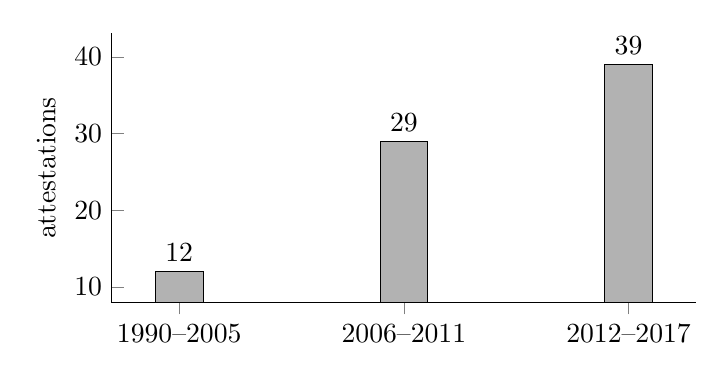
\begin{tikzpicture}
  \begin{axis}[
    axis lines*=left,
    bar width=4ex,
    ybar,
    symbolic x coords = {1990–2005,2006–2011,2012–2017},
    xtick = data,
    nodes near coords,
    ylabel = {attestations},
    height=5cm,
    width = 9cm,
    enlargelimits=0.15,
  ]
  \addplot [draw=black,fill=black!30!white] coordinates {(1990–2005,12) (2006–2011,29) (2012–2017,39)};    
  \end{axis}
\end{tikzpicture}
\caption{COCA evidence that use of \textit{I'm good} `No thanks' has increased steadily between 1990 and 2017\label{fig:rickford:6}}
 \end{figure}

Secondly, investigation of the COCA corpus showed that while this usage may have originated in response to offers of food or drink, this is not the only appropriate context for its use. In fact, only 25\% (25/80) of the examples of \textit{I'm good} `No' in the IG COCA search are a response to offers of food or drink.  This is important because the prosecution had suggested that the agent's use of \textit{I'm good} was not an appropriate context for signaling `No' since it was not in a social setting in which food or drink was being offered. However, in light of the COCA evidence, where a great majority of the \textit{I'm good} `No' examples do \emph{not} involve offers of food or drink, the suggestion that this use of \textit{I'm good} is restricted only to situations involving offers of food or drink is not persuasive.

Thirdly, the COCA corpus helped call into question the Prosecution's claim that Tamika does not choose the familiar and customary phrase of negation, \textit{No, I'm good thanks}, opting significantly to omit the operative word \textit{No} when she says \textit{I'm good}. This statement by the prosecution went against the evidence of the IG COCA corpus that while 54\% (43/80) of the attestations of \textit{I'm good} `No' include a preceding \textit{No} or other explicit negative, as in \REF{ex:rickford:10}, another 45\% (37/80) of them include no explicit negative, as in \REF{ex:rickford:11}.

Fourthly, while \textit{I'm good} is the primary way of signaling `No' in the  \textit{I'm \_\_\_\_} frame, the COCA corpus showed that \textit{I'm okay}, \textit{I'm fine} and \textit{I'm cool} are other alternatives, sometimes used in conjunction with or in place of \textit{I'm good}:

\ea%12
    \label{ex:rickford:12}
   “Do you want something to eat?” she calls. “\textit{Nah,~I'm~cool}. I grabbed a burger on the drive.” (Jeff P. Jones, Antioch Review, 2015, vol. 73, no. 3, p. 495--512, FICTION genre)
\z

Outside of the COCA corpus, there is an interesting recent TV example in which MSNBC reporter Rachel Maddow reads this segment of the News (exhibit \#4):

\ea%13
	\label{ex:rickford:13}
The individual who asked for the secret filing declined to identify himself or his client and replied “I'm OK” when offered a reporter's business card to remain in touch. (MSNBC 10/25/18, 9:40 pm)
\z

Maddow goes on to perform a mock re-creation\slash elaboration of the scene, using \textit{I'm OK} `No':  

\ea%14
    \label{ex:rickford:14}
 \# “Well, I know you don't want to talk now, but can I give you my card if you should like to talk at some point in the future?" “\textit{Yeah,} \textit{I'm} \textit{OK}.  I don't need your business card.  If I go home with your business card in my pocket, I'll disappear.  Ha ha.  In fact, I was never even here!” (MSNBC 10/25/18, 9:40 pm)
\z

   
Note that the presence of \textit{Yeah}  in the \textit{I'm good}  or \textit{I'm OK}, etc. frame does not, as example \REF{ex:rickford:14} shows, necessarily signal assent to the request or offer to which it is a response, especially when an offer or request is repeated, as is frequently the case, and when that  request or offer is unpleasant, or potentially threatening the responder's “face,” sense of appropriateness, health or freedom.  This is certainly the case with the “pat down” that the DEA agent sought permission to do.

Bearing these points in mind, I was able to call into question the observation of the Prosecution in their Amended Prosecution Response that in this exchange, Tamika's response of \textit{I'm cool} to the agent's \textit{Okay?} “gave ultimate completeness to the consent that she gave to his request to search her”:

 
\ea%15
\label{ex:rickford:15}
DEA Agent: You give me permission just pat you down? \\
Tamika: I’m good. \\
DEA Agent: Okay?\\
Tamika: I'm cool, yeah.
\z

        
This is certainly a possible interpretation, but in light of the following example \REF{ex:rickford:16} from the COCA corpus, it is also possible to see Tamika reaffirming the \textit{I'm good} `No' of her first response.  The presence of \textit{Yeah} here is most probably a repudiation of her initial negative \textit{I'm good} as it is in example  \REF{ex:rickford:16} below.  And indeed, in context (a second response to a less than pleasant request) this is the more likely interpretation. 

\ea%16
  \label{ex:rickford:16}
JOSH-ELLIOTT-1-AB\#~(Off-camera) I do want to say, Melissa and I shared a car afterwards, we're going back to the hotel and she says, do you want some Advil? And she'd done it before, and I said, no, you know, I'm tired, I have an empty stomach,~\textit{I{}'m}~\textit{good.}~I'll get some later. She said, you're sure? I said, yeah, \textit{I'm} \textit{good}, and I forgot to take some.  [from Josh and Melissa on Wipeout, ABC, SPOKEN genre, 2011]
\z
         
In addition to the COCA corpus, we also selected 75 Twitter examples from selected dates in 2015, 2016 and 2018 in which \textit{I'm good} was used in the sense of `No (thanks)', as in this example:

 \ea%17
    \label{ex:rickford:17}
 You think I work my ass off to take you out on a date?  Smoke you out?  Buy you shit?    Nah b, I enjoy my own company.  \textit{I'm} \textit{good.} (BamBriaan, Nov 6, 2015)
\z
 

Twitter is a very “oral” medium, which is huge and constantly growing.  In this medium, the innovative usage is extremely frequent.  It is also interesting that the percentage of examples in which \textit{I'm good} is preceded by \textit{No}, \textit{Naw} or another negative is about the same as in the COCA corpus, 52\% (39/75).  About half of the time (48\%, 36/75) \textit{I'm good} retains its negative force without an accompanying overt negative form, suggesting, once again, that Defendant Tamika did not need to use an overt \textit{No} for her \textit{I'm good} to mean `No (thanks)'.

One perhaps relevant observation is that most of the Twitter examples come from African Americans.  (Twitter examples often include a photo of the sender.) It is not my contention that \textit{I'm good} `No' is a distinctly African American usage; the examples in COCA demonstrate clearly that while it a relatively new usage, it is used by a wide cross section of the American public.  However, Twitter is extremely popular among African Americans, and the frequency with which the \textit{I'm good} `No' tokens come from African Americans suggests that this usage would not have been unfamiliar to Tamika.   Very likely it is something she encountered and perhaps used frequently in talking with and reading Twitter posts from other African Americans.

Three other observations about the Twitter examples that might be of more interest to linguists than the court are these.  Firstly, and this may be related to the 140-character restriction of Twitter, many of the examples do not contain the Yes\slash No questions or assertions to which they are a response.  Sometimes these are evident in the tweets of one or more other persons to which they represent a response.  Secondly, a number of idiomatic spinoffs of \textit{I'm good}, have emerged in this medium.  One is \textit{I'm good, luv, enjoy} (adding a sarcastic twist) as in:

\ea%18
\label{ex:rickford:18}
You done pissed me off for the LAST time.  \textit{I'm good luv, enjoy}! * (ayootw33t,  Nov 3, 2018)
\z

Another is the use of \textit{I'm good} with a following prepositional phrase, as in:

\ea%19
    \label{ex:rickford:19}
 Too much fake love at FAMU*  *\textit{I'm good off all that} * (JoseTheTre Oct 29, 2018)
\z  
  
  
Thirdly, the use of \textit{I'm good} to reject offers that are less than pleasant and potentially self-incriminating (as was true of the body search invitation Tamika declined) is evident in examples like this one, where the tweeter suggests that the \textit{free tattoo} might result in hepatitis:

\ea%20
\label{ex:rickford:20}
Some guy just messaged me a video on FB of him sitting at a coffee table with a tatoo machne, made it buzz and said, “Come and get a free tatt” ...“I'm good on hepatitis, my dude”  (\_frvitbat, Oct 29, 2018)
\z

So how did this evidence pan out for Tamika’s case? In consultation with her lawyer, she opted to plea bargain rather than go to trial, as happens in more than 96\% of U.S. cases, for complex reasons, including the evidence of her sister’s case.  However, the lawyer submitted my evidence for the usage of \textit{I'm good} to mean `No' in a final, extended “Expert Notice” to the court, drawing on the COCA evidence and the evidence from the Twitter examples.  This apparently persuaded the prosecution to agree to more favorable terms (maximum 3 years, including the one already served) for the plea bargain of 10 years that would otherwise have been the case. As a result, her final sentence was 2 years, rather than 10, including time served, demonstrating another way in which linguistic analysis based on corpora can be very impactful in applied contexts.

\section{Summary and conclusion: Towards online corpora of Caribbean Languages}

As the above six examples have shown, online corpora can provide an invaluable, sometimes \textit{essential} resource for the study of linguistic variation and change, in theoretical, descriptive, and applied contexts.  They are particularly valuable when they are online and publicly available, allowing our analyses to be replicated and validated.

In the English-speaking Caribbean, we already have multiple sources for these kinds of corpora, although they are at different levels of public availability and accessibility:

\begin{itemize}
\item  Creole recordings already in the Jamaican Language Unit (\textit{Jumieka Langwij Yuunit}), University of the West Indies, Mona, for a long time under the direction of Hubert Devonish, now directed by Joseph Farquharson.
\item  ICE (International Corpus of English) Jamaica -- by design, mainly acrolectal/standard. 
\item  CCJ (Corpus of Cyber Jamaican) -- all levels -- Christian Mair, U Freiburg, Mair adds (in an email from 5/16/19) that the best and most comprehensive showcase of these data is a PhD thesis produced by Andrea Moll (see \citealt{Moll2015}). 
\item  Several hundred Creole recordings and transcripts I have from Guyana, Jamaica and Barbados (many made by me, a native Guyanese, others by local linguists from Guyana and Jamaica).   Most of these will be available in digital form via Stanford University Library. 
\item  Don Winford’s recordings/transcripts from Sranan Tongo, Belize Creole, Guyanese Creole, and Trinidadian Creole, which he has promised to contribute to online corpora being assembled by Bettina Migge, at the University of Dublin. 
\item  Peter Patrick’s Jamaican recordings/transcripts.  Of these he notes (email of 5/20/19) that “The Veeton recordings from 1989- 90 include more than 100 hours of interviews with about 75 different individuals, many in repeat recordings, plus a series of family and youth-club recordings”. I also made a small series of recordings in rural locations in 1991 - principally St. Thomas and Hanover, when I was trying to revisit as many remote sites where Fred Cassidy and David DeCamp made recordings.
\item  Veronique Lacoste (email of 5/28/19) notes that she has about {\textasciitilde}10GB of Jamaican Creole child language data, mostly recorded in schools. 
\item  Other sources: Pauline Christie, Walter Edwards, Shelome Gooden (see \citealt{Gooden2003}), Hazel Simmons-McDonald, Velma Pollard, Ian Robertson, and the many others who have done field work on anglophone Caribbean varieties may be willing to contribute recordings from their collection, and should be actively approached about doing so.
\end{itemize}

There should be similar efforts for the French-speaking Caribbean, the Span\-ish-speaking Caribbean, and so on.  Indeed, there undoubtedly already are.  For instance, Nicte Fuller Medina has corpora of Belizean Spanish as well as English\slash Creole on her Language, Culture and History project website.\footnote{\url{https://nfullerm.wixsite.com/website/research}}

Building on and using these resources will not be without challenges. We would need to determine how to collect, catalog, digitize, and safely store recordings and transcripts of Caribbean language varieties, deciding on real names or pseudonyms depending on available permission forms and local IRB (Institutional Review Board) rules. We’d also need to decide about placement: that is what would go where, whether there would be sharing between sites, and so on. Furthermore, we’d need to develop tools for the automatic analysis of digital recordings and transcripts that can handle Caribbean lexicon, phonology, and morphosyntax, along the lines that Shelome Gooden and others have begun to pioneer. And while there are numerous necessary steps to this process, we do have the people who can make it happen. 

In order to accomplish this, we could perhaps start with small meetings (facilitated by funding from agencies like the National Science Foundation) of key players to discuss the issues. We could also get the advice or involvement of experts like Tyler Kendall (University of Oregon, and the developer of two web-based language archives, including CORAAL)  and Christian Mair.\footnote{\url{https://blogs.uoregon.edu/lvclab/people/tyler-kendall/} and \url{https://www.researchgate.net/profile/Christian_Mair}}   But we need to begin soon, because one of the best ways we can honor pioneer linguists of the Caribbean, before they pass on, is by equipping their successors with online corpora of Caribbean languages.  They are invaluable, indeed essential tools for 21\textsuperscript{st} century Linguistics.


\section*{Acknowledgments}
I am grateful to the following Stanford students for assistance in the preparation of this paper: Mea Anderson, Jane M. Boettcher, Susan Chang, Julia Gong, and Zion Ariana Mengesha.  And as always, for the encouragement and support of Angela Eunice Rickford, my intellectual companion for more than 50 years.   I also thank the two anonymous referees for their helpful comments on an earlier draft.

\section*{Abbreviations}
\begin{tabularx}{\textwidth}{@{}lQ@{}}
\textsc{AAVE} & African American Vernacular English  \\
\textsc {ASR}& Automated Speech Recognition \\
\textsc {VOC} & Voices of California \\
\textsc {WER} & Word Error Rate   \\
\textsc {COCA}& Corpus of Contemporary American English\\
\textsc{CORAAL} & Corpus of Regional African American Language\\
\textsc{ICE} & International Corpus of English\\
\textsc {IRB} & Institutional Review Board\\
\end{tabularx}

\largerpage
\printbibliography[heading=subbibliography,notkeyword=this]
\end{document}
